

\documentclass[a4paper]{article}

\usepackage{amsmath}
\usepackage{hyperref}
\usepackage{biblatex}
\usepackage{enumerate}
\usepackage{graphicx}
\usepackage{stmaryrd}
\usepackage[dvipsnames]{xcolor}
\usepackage{listings}
\usepackage{caption}
\usepackage{subcaption}
\usepackage{booktabs}
\usepackage{float}

\addbibresource{refs.bib}

\begin{document}

\author{Ola Bratt \\
  \href{mailto:ola.bratt@gmail.com}{ola.bratt@gmail.com}
  \and
  Patrick Attimont \\
  \href{patrickattimont@gmail.com}{patrickattimont@gmail.com}
}

\title{DAT565/DIT407 Assignment 4}
\date{2024-02-15}

\maketitle

This paper is addressing the assignment 3 study queries within the \emph{Introduction to Data Science \& AI} course, DIT407 at 
the University of Gothenburg and DAT565 at Chalmers. The main source of information for this project
is derived from the lectures and Skiena~\cite{Skiena:2024}. Assignment 4 is about correlation and linear regression.

\section*{Problem 1: Splitting the data}
The dataset is large enough to be separated into a train and a test set. We use the function \verb|train_test_split| with a test size of 0.2 to split the data frame, and then extract the X and y (LEB) variables from the train and test sets.


\section*{Problem 2: Single-variable model}
To identify the variable with the strongest linear relationship with the target variable, we use the \verb|corr| function specifying the Pearson method to get a correlation matrix between all the variables (Fig~\ref{fig:pearson_correlation}), and take the column corresponding to the target variable.

The variable with the highest absolute pearson coefficient is the Human development index, with a value of 0.92.
Fig~\ref{fig:reg_human_development_index} shows the linear regression applied on the test set, using the model built on the train set.
The model has a slope of 48.2, an intercept of 37.3, and a determination coefficient of 0.87. These values obviously slightly change depending on the seed used to split the data.
The mean squared error between the test and predicted sets is 9.45.

The human development index measures a country's social and economic development. As specified on UNDP's website (\cite{UNDP:2023}), it is calculated based on the following factors: life expectancy, education, and standard of living.
Thus the strong relationship between the two variables comes from the fact that life expectancy at birth is used to calculate the human development index.


\begin{figure}[H]
  \begin{center}
    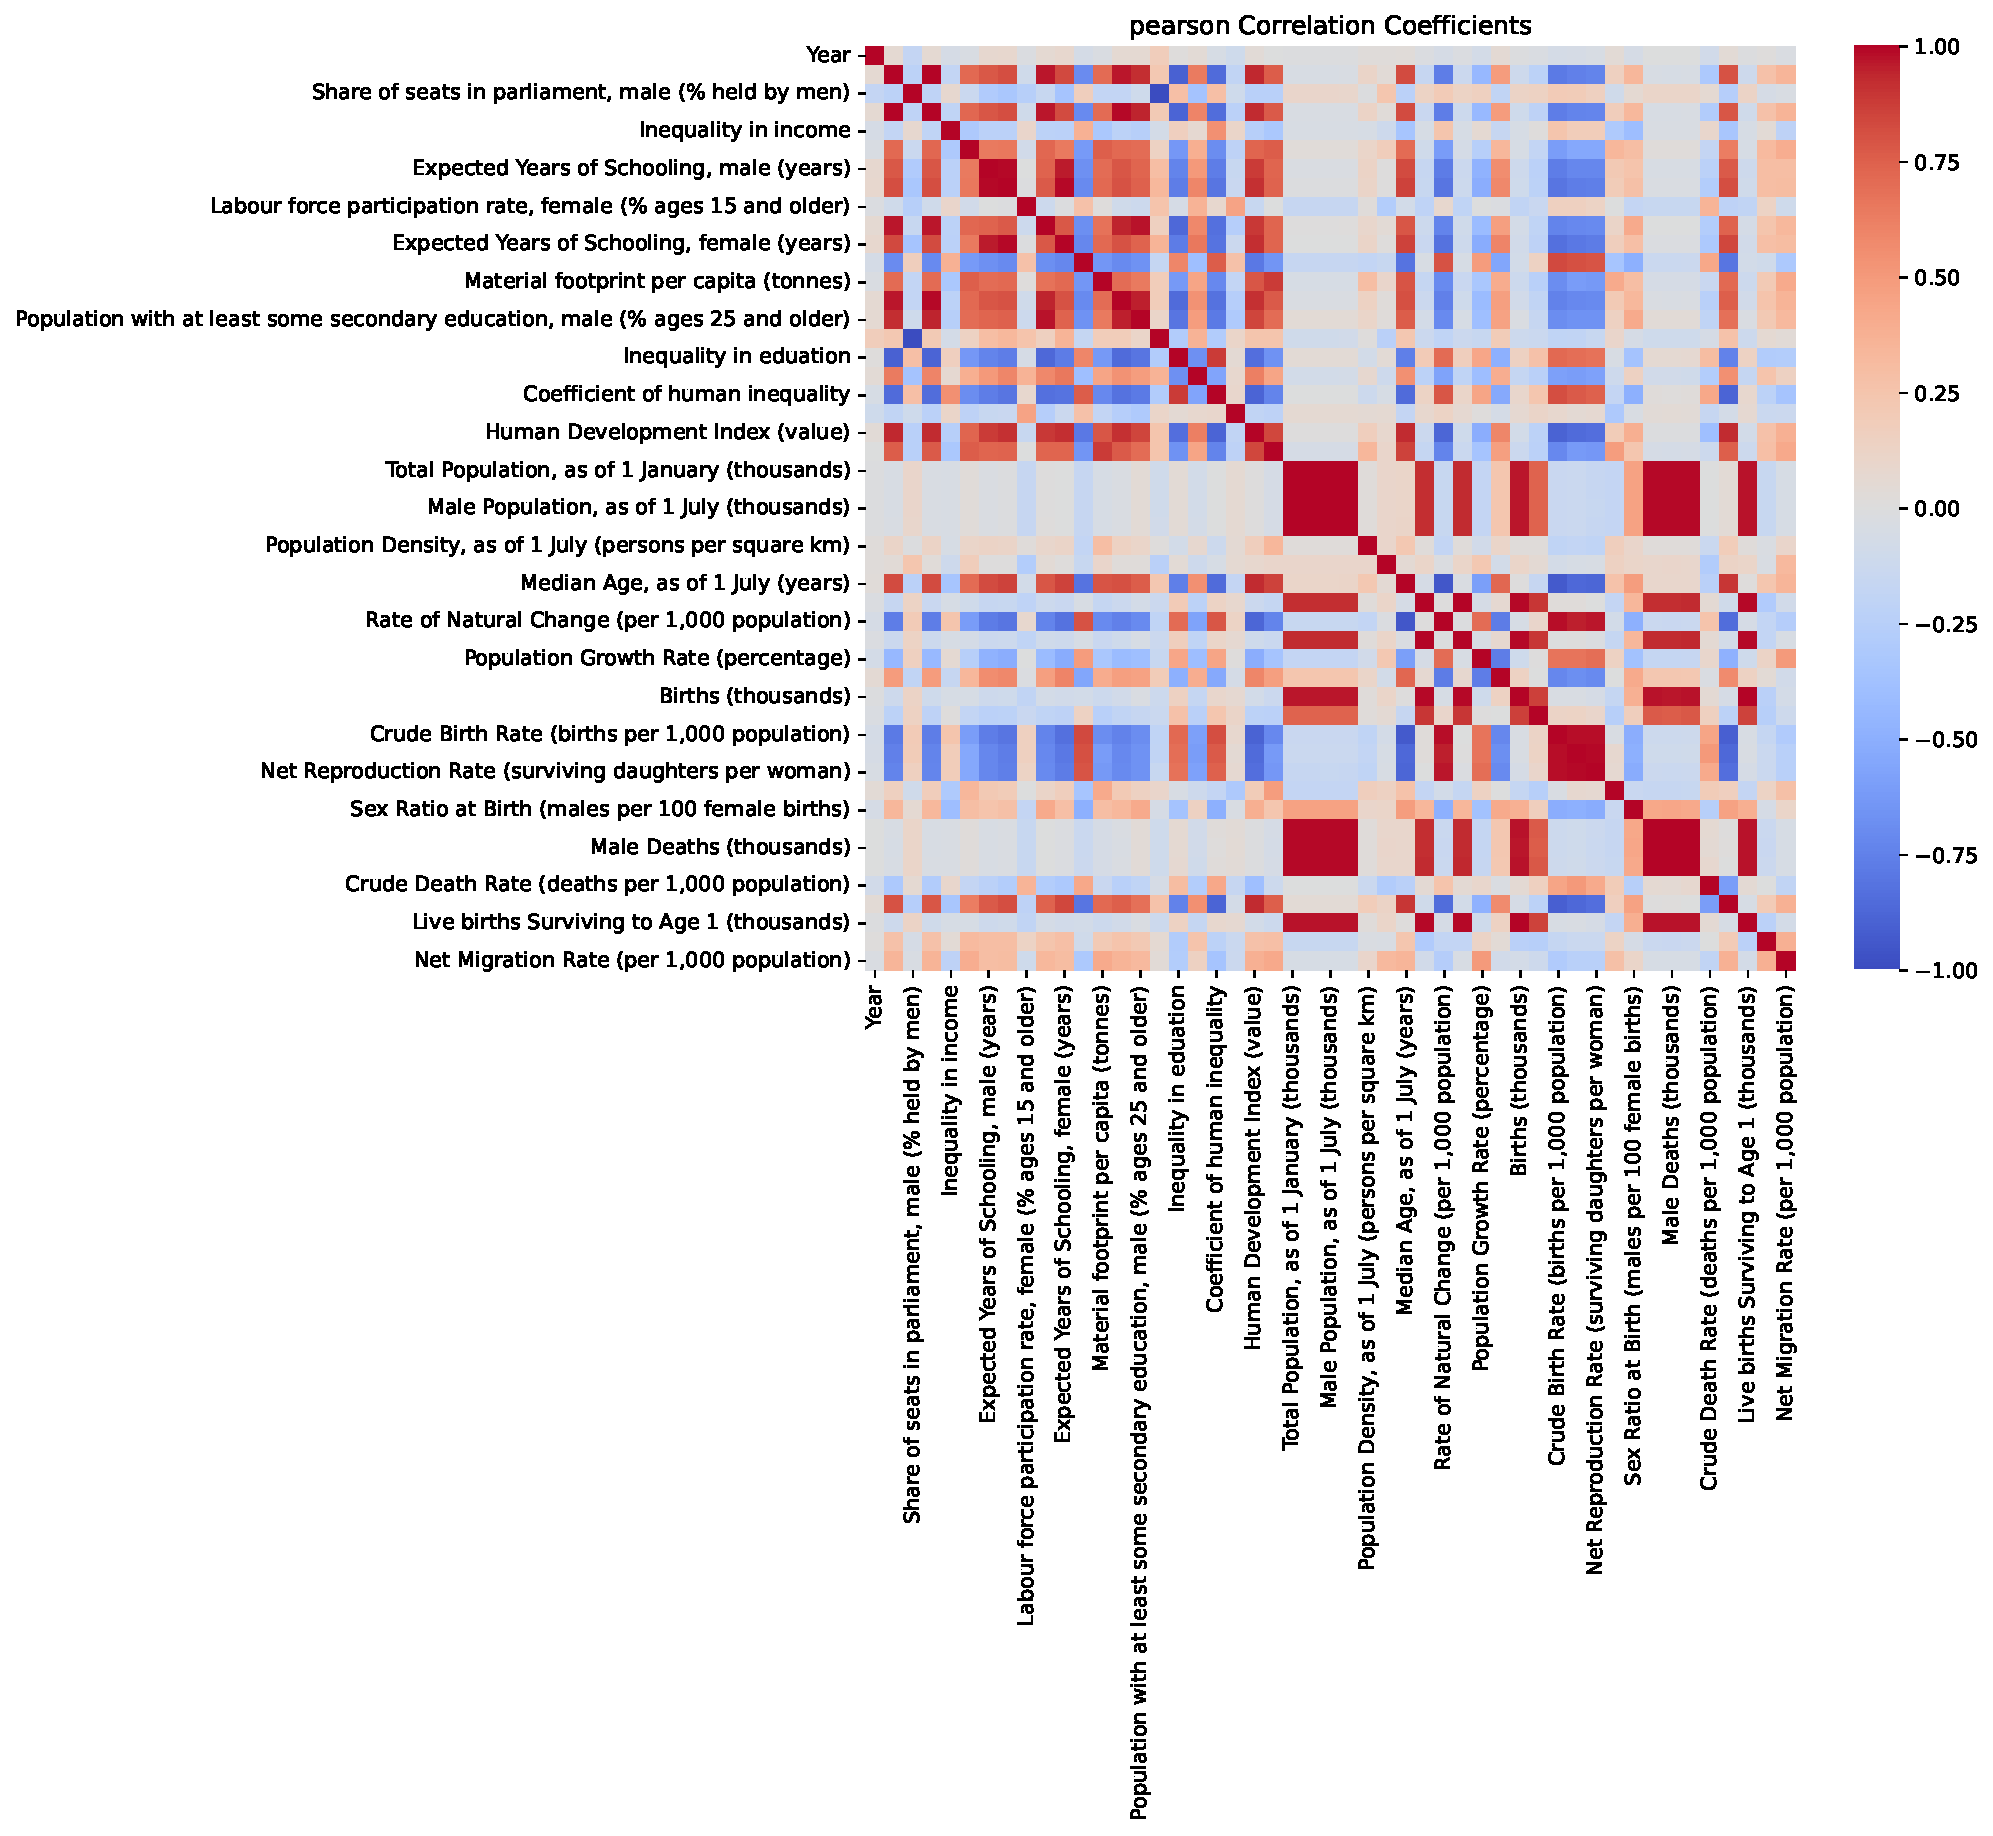
\includegraphics[width=\textwidth]{ola/pearson_correlation.pdf}
    \caption{Correlation Pearson}
    \label{fig:pearson_correlation}
  \end{center}
\end{figure}

\begin{figure}[H]
  \begin{center}
    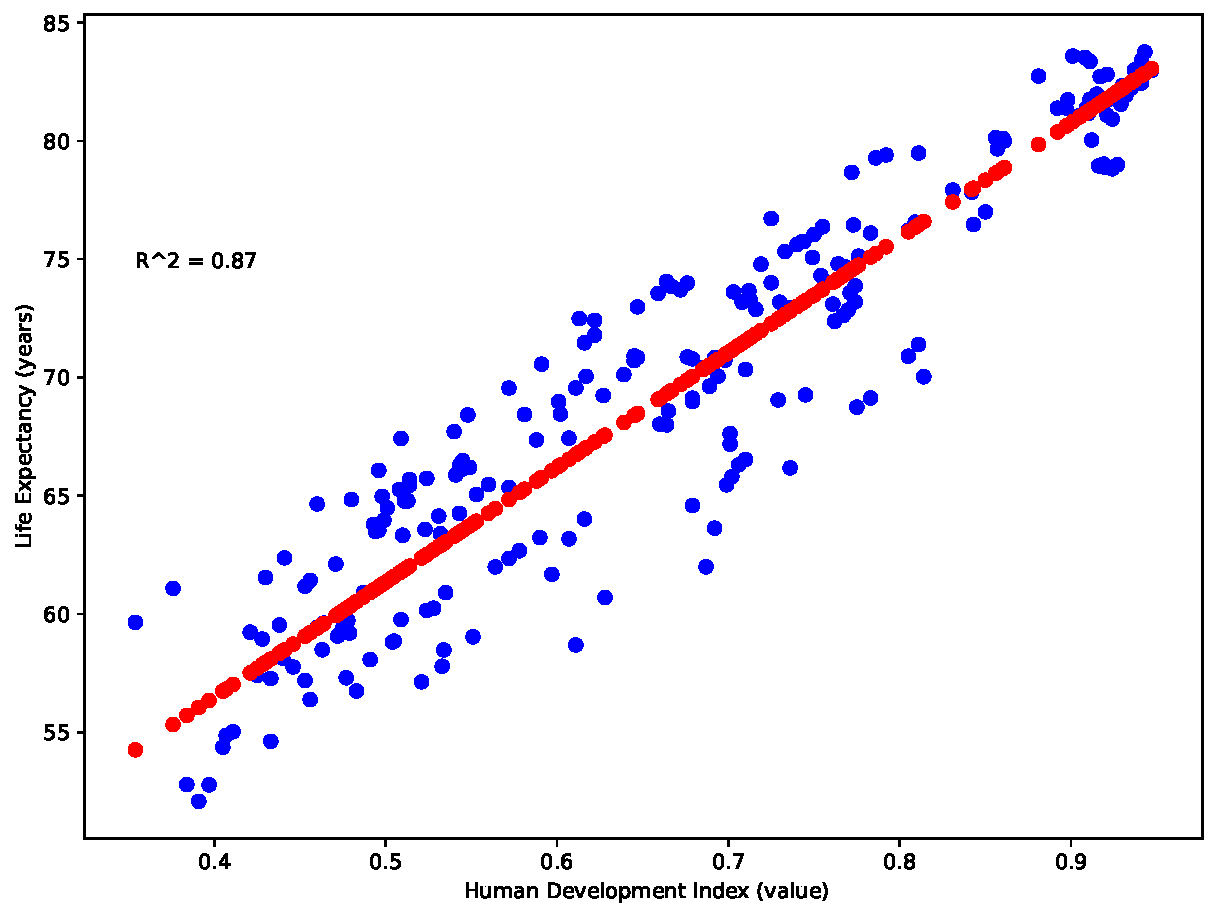
\includegraphics[width=\textwidth]{ola/_linear_regression_human_development_index_(value).pdf}
    \caption{Linear Regression Human Development Index (value)}
    \label{fig:reg_human_development_index}
  \end{center}
\end{figure}

\section*{Problem 3: Non-linear relationship}

To explore variables with non-linear relationships, we initially assess Spearman correlation coefficients, Figure~\ref{fig:spearman_correlation}. 
Initially, we eliminate the variable exhibiting the strongest Pearson correlation, namely 'Human Development Index (value)'. Subsequently, we examine the Spearman correlation.

Our analysis reveals that 'Median Age, as of 1 July (years)' exhibits the most robust Spearman correlation. Subsequently, 
we develop a linear model using this variable to determine the mean squared error, which amounts to 13.58, Figure~\ref{fig:reg_median_age}.

Next, we apply transformations to the variable using logarithmic, square root, and reciprocal functions, respectively  Figure~\ref{fig:linear_transformation}. 
For each transformation, we train a linear model to ascertain the resulting mean squared error. The logarithmic transformation yields the lowest mean squared error, measuring 11.52.  Figure~\ref{fig:reg_median_age_log}.

Before transformation, the Pearson correlation registers at 0.898, while after transformation, it increases marginally to 0.913.


\begin{figure}[H]
  \begin{center}
    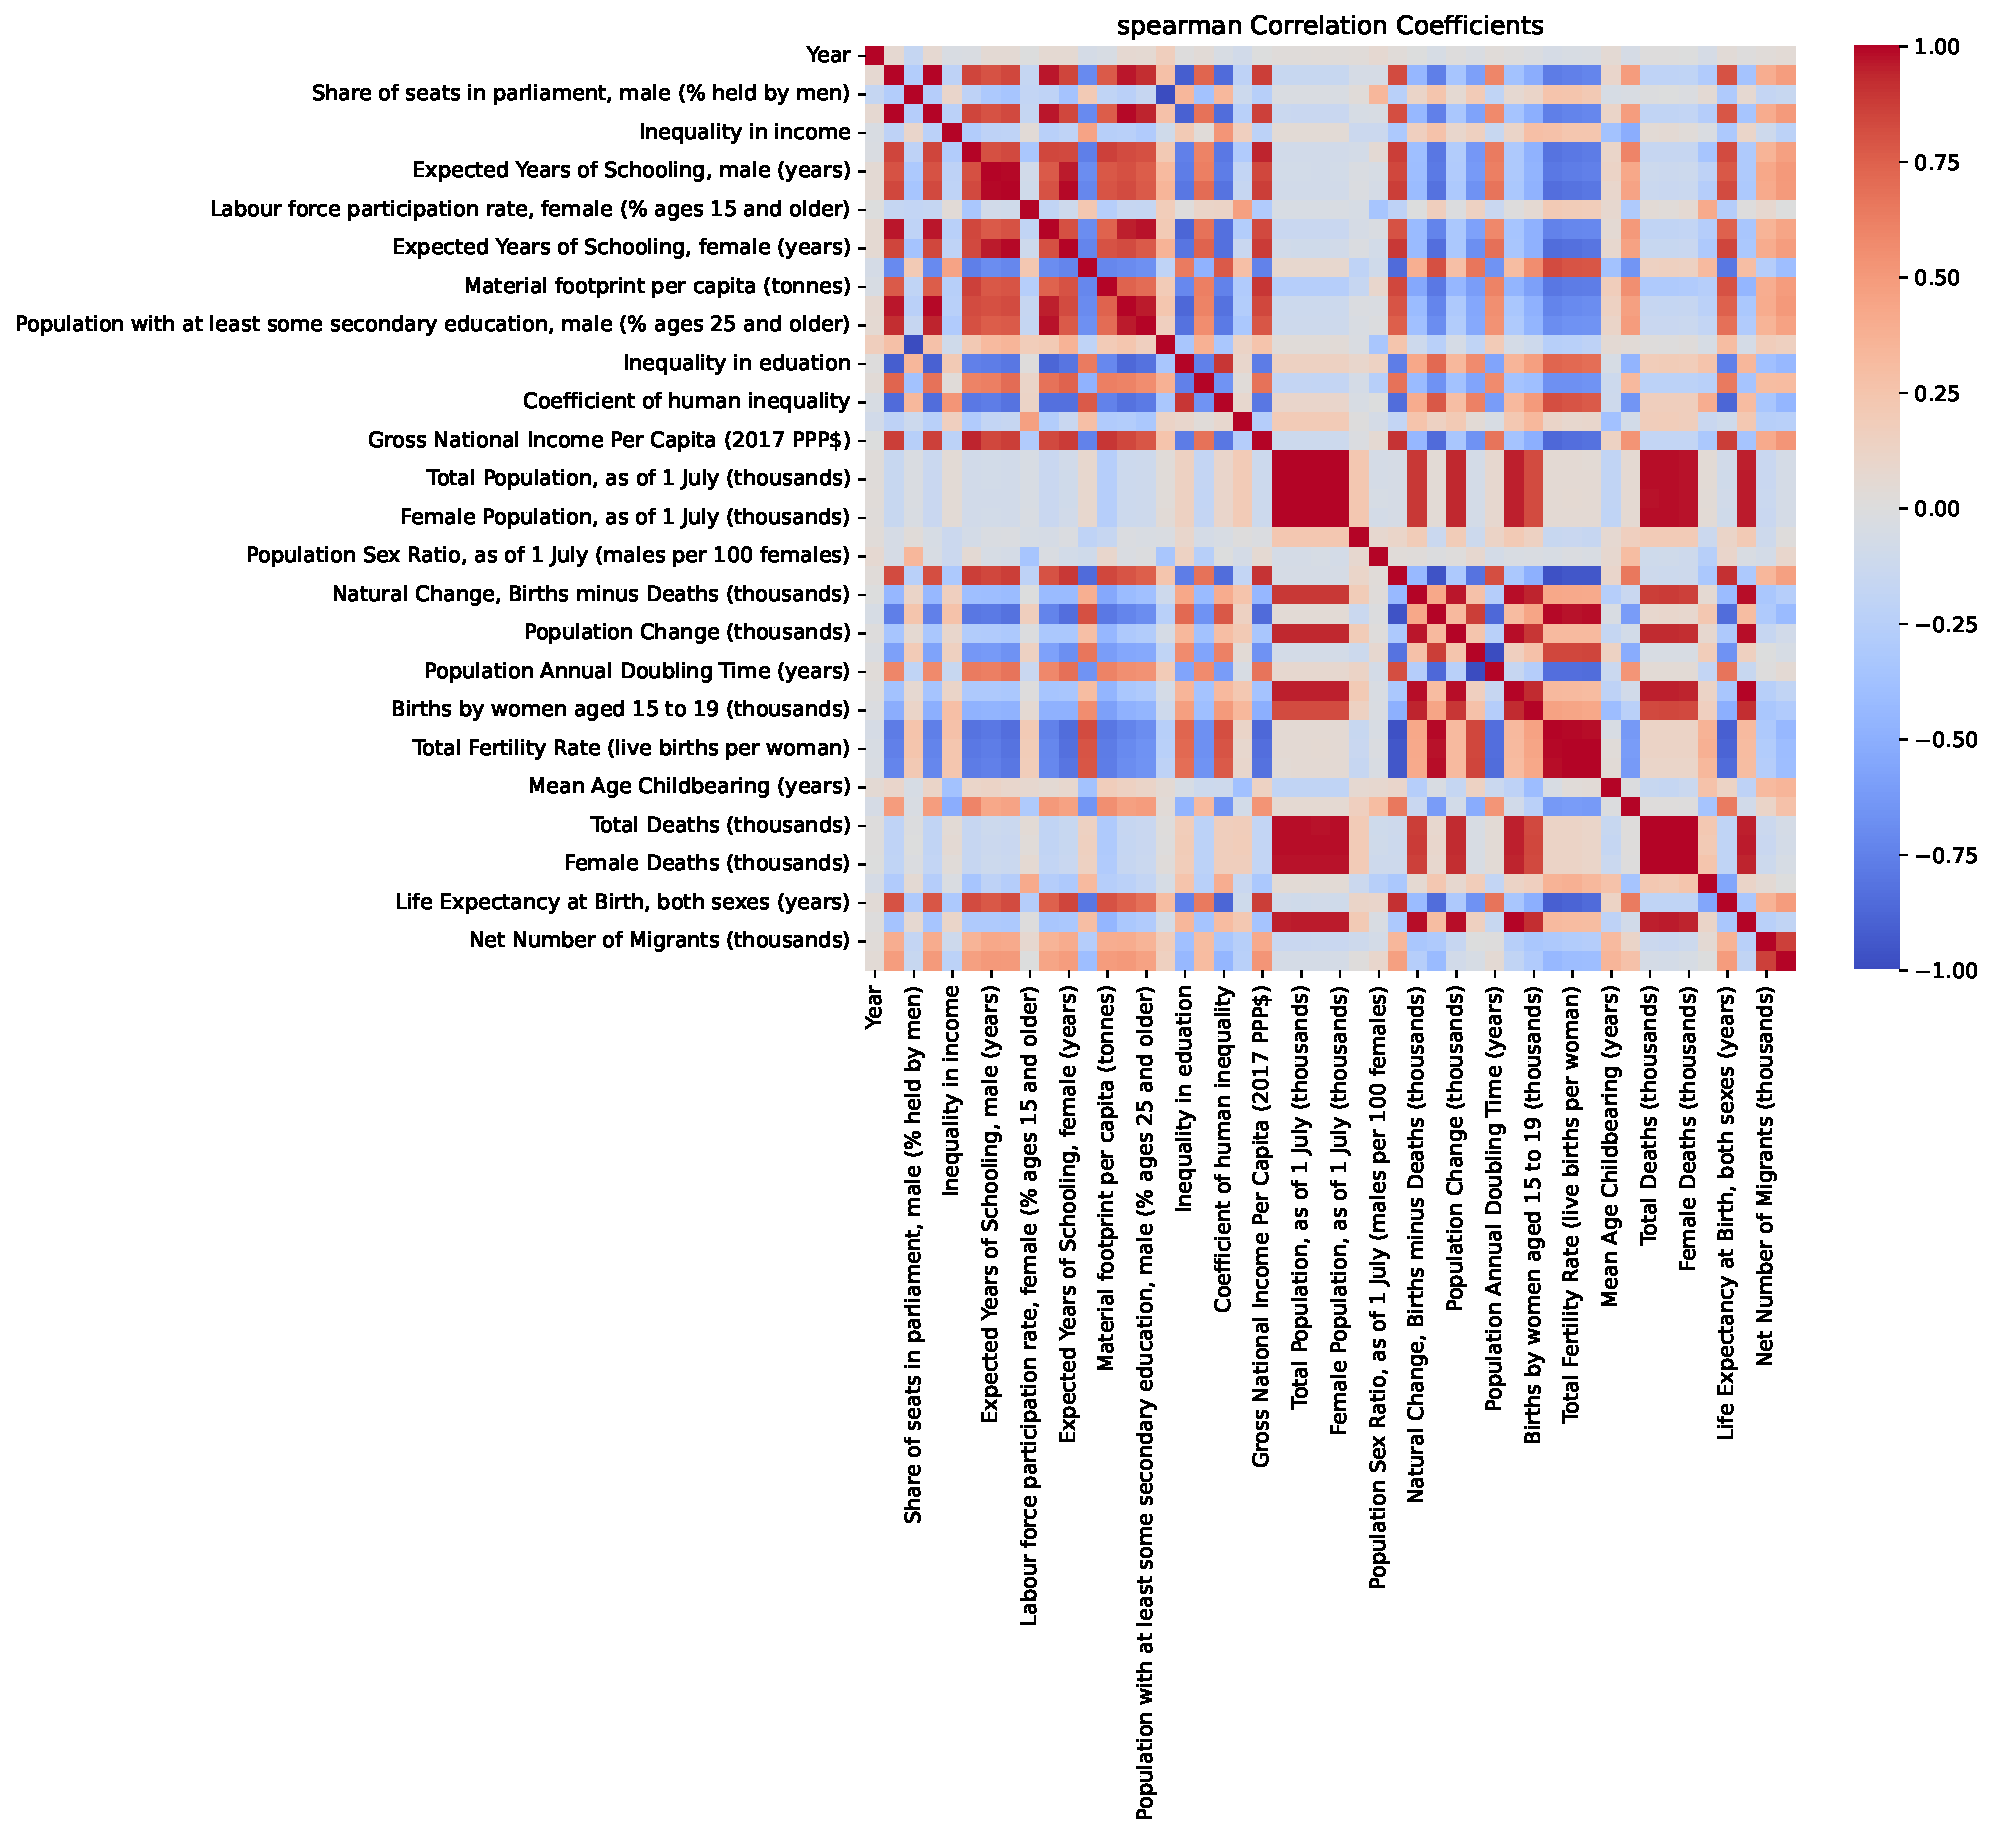
\includegraphics[width=\textwidth]{ola/spearman_correlation.pdf}
    \caption{Correlation Spearman}
    \label{fig:spearman_correlation}
  \end{center}
\end{figure}


\begin{figure}[H]
  \begin{center}
    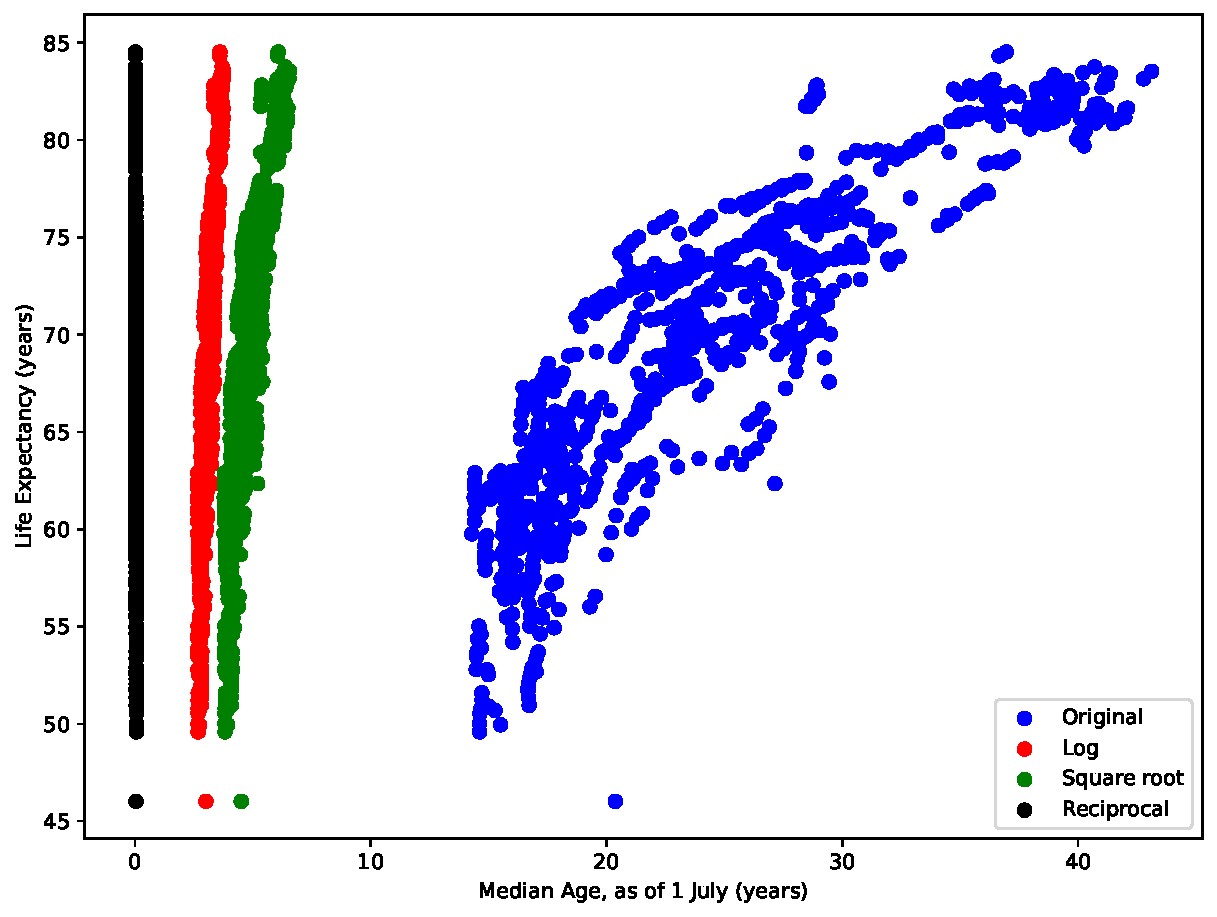
\includegraphics[width=\textwidth]{ola/linear_transformation.pdf}
    \caption{Linear transformation}
    \label{fig:linear_transformation}
  \end{center}
\end{figure}

\begin{figure}
  \centering
  \begin{subfigure}[a]{\textwidth}
      \centering
      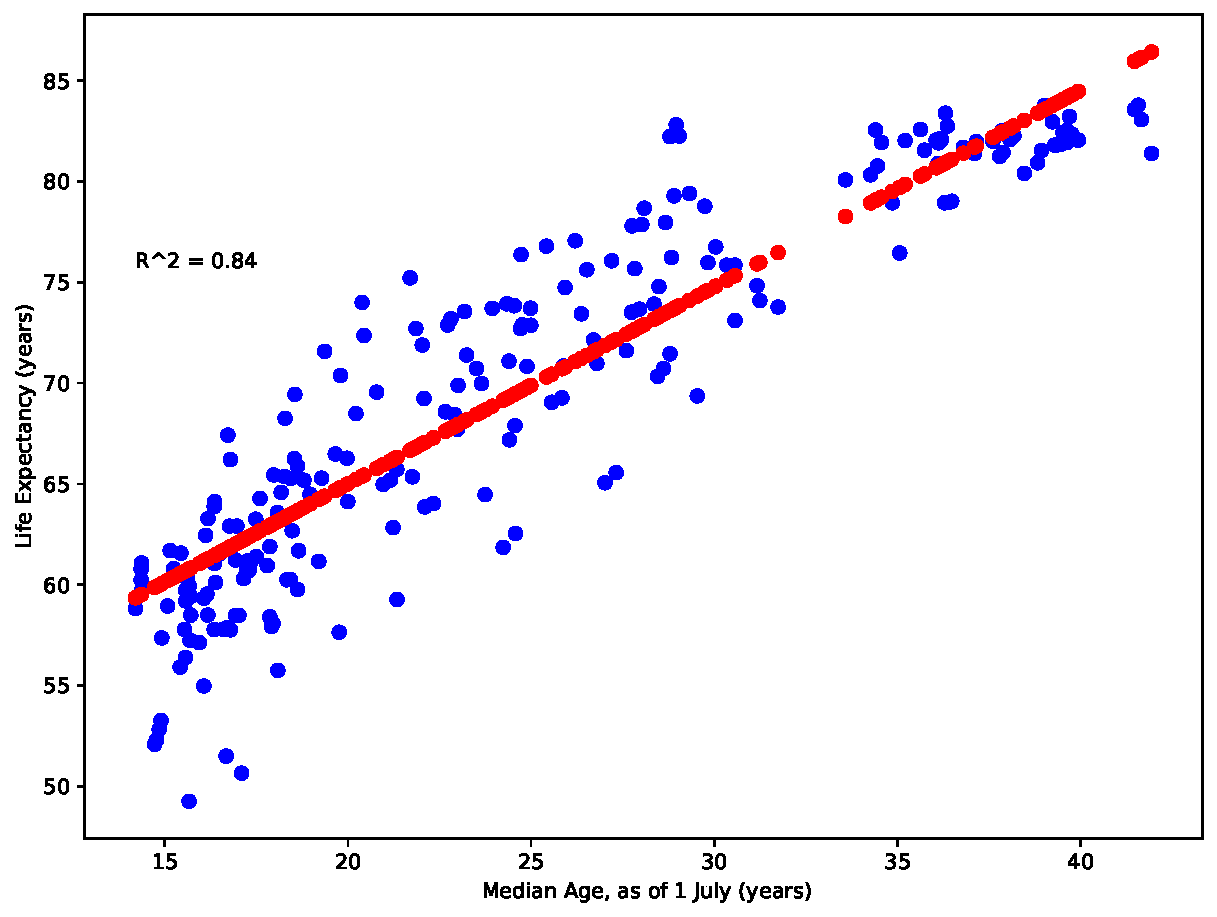
\includegraphics[width=\textwidth]{ola/_linear_regression_median_age,_as_of_1_july_(years).pdf}
      \caption{Linear Regression Median Age (original)}
      \label{fig:reg_median_age}
  \end{subfigure}
  \vfill
  \begin{subfigure}[b]{\textwidth}
      \centering
      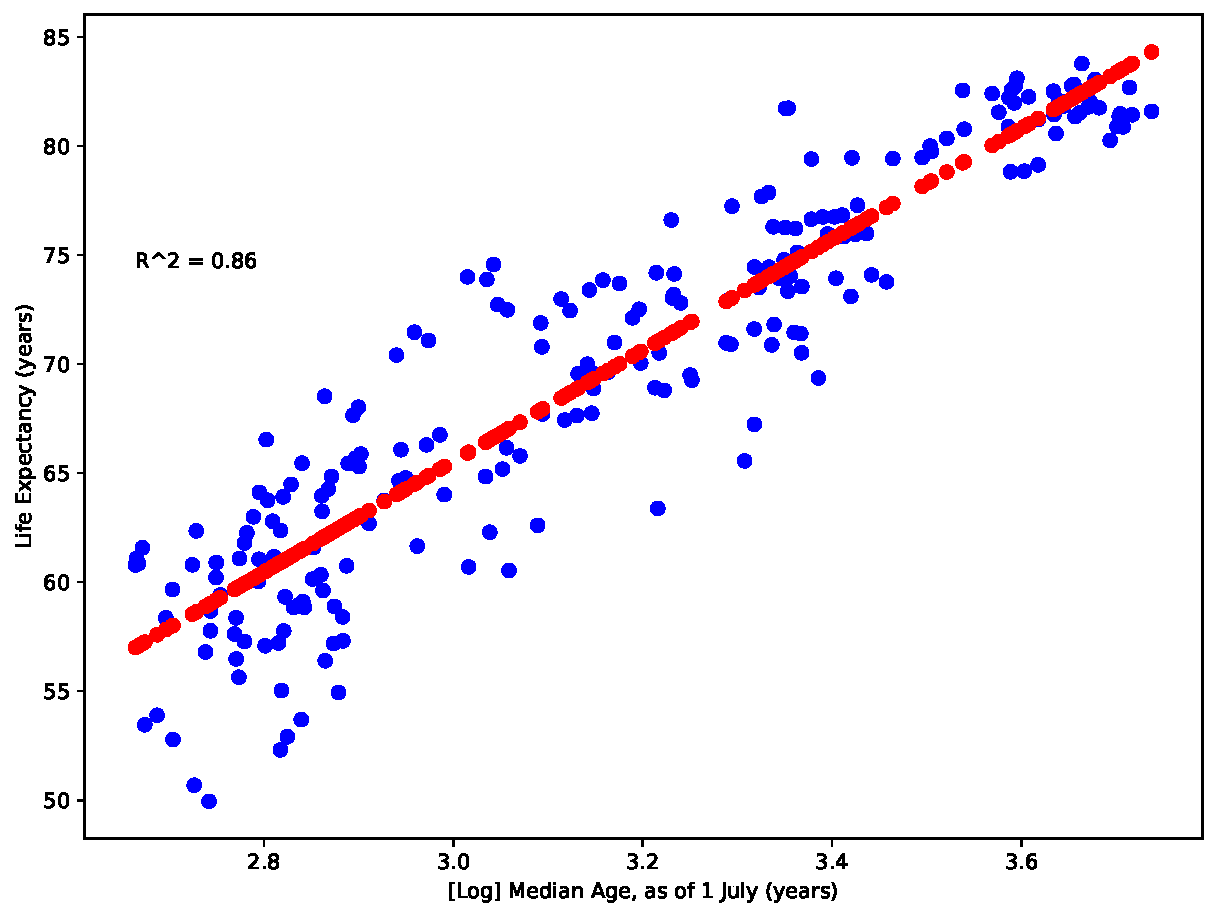
\includegraphics[width=\textwidth]{ola/[log]_linear_regression_median_age,_as_of_1_july_(years).pdf}
      \caption{Linear Regression Median Age (log)}
      \label{fig:reg_median_age_log}
  \end{subfigure}
  \caption{Linear Regression Median Age}
  \label{fig:linear_regression_median_age}
\end{figure}

\section*{Problem 4: Mulitple linear regression}

We utilized Spearman correlation analysis as a method to distinguish variables exhibiting strong correlations with our target. 
By setting a predetermined threshold, we aimed to identify variables exerting significant influence on the target variable.

After conducting experiments with different threshold values, we observed that a threshold of 0.85 yielded satisfactory results, achieveing a balance between inclusivity and relevance.

The variables identified through this process are: 

\begin{verbatim}
  Expected Years of Schooling for females 
  The Coefficient of Human Inequality 
  Gross National Income Per Capita for the year 2017
  Median Age as of 1 July
  Rate of Natural Change per 1,000 population
  Crude Birth Rate measured in births per 1,000 population
  Total Fertility Rate denoting live births per woman
  Net Reproduction Rate denoting surviving daughters per woman.
\end{verbatim}

Upon conducting a multiple linear regression analysis on the selected variables, we obtained a mean squared error of 2.03, indicative of the model's predictive accuracy. 
Additionally, the model achieved an R-squared score of 0.95, suggesting a high degree of variance explained by the model.

The coefficients derived from the regression model provide insights into the strength and direction of the relationships between the independent variables and the target variable.
The intercept of the model is 78.24 and the coefficients for the model are as follows:
\begin{verbatim}
  19
  -571
  243338
  61
  1.7
  -2.1
  1.9
  3
\end{verbatim}



\newpage


\printbibliography

\section*{Appendix: Source Code}

\lstset{
  language=Python,
  basicstyle=\ttfamily,
  commentstyle=\color{OliveGreen},
  keywordstyle=\bfseries\color{Magenta},
  stringstyle=\color{YellowOrange},
  numbers=left,
  basicstyle=\footnotesize,
  breaklines=true,
  postbreak=\mbox{\textcolor{red}{$\hookrightarrow$}\space}
}


\lstinputlisting{ola/assignment4.py}

\end{document}
